\documentclass[10pt]{report}

\usepackage[utf8]{inputenc}
\usepackage[T1]{fontenc}
\usepackage{latexsym} 
\usepackage{bbm}            
\usepackage{graphicx}         
\usepackage{epsfig}           
\usepackage{amsmath}          
\usepackage{amsfonts}
\usepackage[english]{babel}

\usepackage{marvosym}
\usepackage{multirow}
\usepackage{colortbl}
\usepackage{tkz-tab}
\usepackage{algorithm}
\usepackage{algorithmic}
\usepackage{fancyhdr}
\usepackage{color}
\usepackage{geometry}
\usepackage{caption}

%
\setlength{\paperheight}{297mm}\setlength{\paperwidth}{210mm}
\setlength{\oddsidemargin}{10mm}\setlength{\evensidemargin}{10mm}
\setlength{\topmargin}{0mm}\setlength{\headheight}{10mm}\setlength{\headsep}{8mm}
\setlength{\textheight}{240mm}\setlength{\textwidth}{160mm}
\setlength{\marginparsep}{0mm}\setlength{\marginparwidth}{0mm}
\setlength{\footskip}{5mm}
\voffset -13mm\hoffset -10mm\parindent=0cm

\newcommand{\qed}{\hfill $\Box$\hfill\\}
\newcommand{\R}{\mathbb{R}}
\newcommand{\C}{\mathbb{C}}
\newcommand{\N}{\mathbb{N}}
\newcommand{\Z}{\mathbb{Z}}
\newcommand{\K}{\mathbb{K}}
\newcommand{\di}{\mathrm{d}}


\begin{document}



\begin{titlepage}
\begin{center}

\textsc{\LARGE Project MNXB01}\\[2cm]

 % Title
    \hrule 
    ~\\
    { \huge \bfseries Swedish climate study\\[0.4cm] }
    
    \hrule
    ~\\[2cm]
    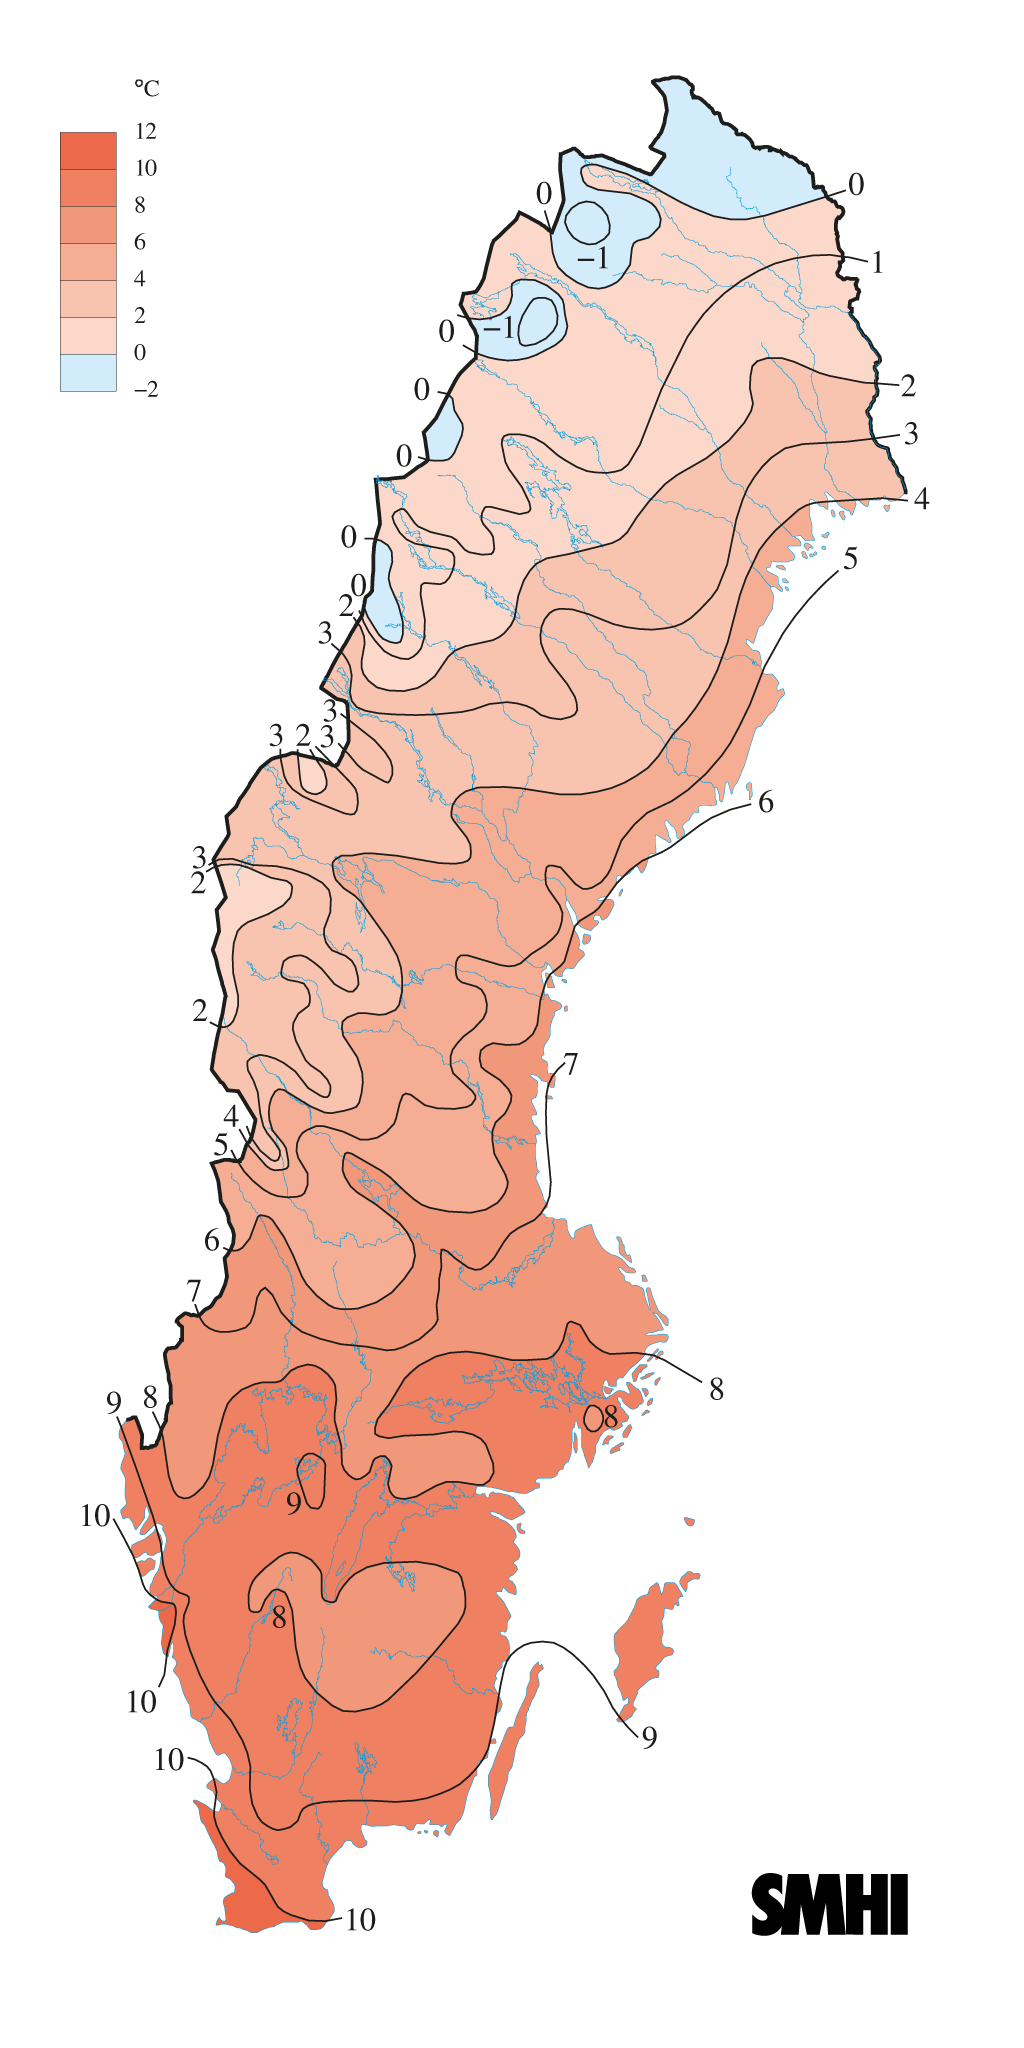
\includegraphics[scale=0.2]{MapSweden.png}~\\[2cm]
\end{center}
 \vfill
 % Author
\begin{minipage}{0.4\textwidth}
 \begin{flushleft} \large
        \textsc{SERNOUX Estelle}\\
        \textsc{SIEMUND Philip}\\
        \textsc{HUYNH Jasmain}\\
        \textsc{LEYGONIE Johan}\\
      \end{flushleft}
\end{minipage}
\begin{minipage}{0.4\textwidth}
 \begin{flushright} \large
       \textsc{06/11/19}
      \end{flushright}
\end{minipage}
\end{titlepage}

\newpage
\tableofcontents

\chapter{Introduction}
The goal of this project is to study Swedish climate via different programms. We have access to various datasheet containing the temperatures at different times, for a bunch of swedish cities. We will be essentially focusing on Lund's weather as we currently live there. We where given some examples of what kind of programm would fit the subject and we decided to code three of the examples and make three up by ourselves. Then we have assigned one or several code to write to each of use and put it in the workplan as following :

\begin{center}
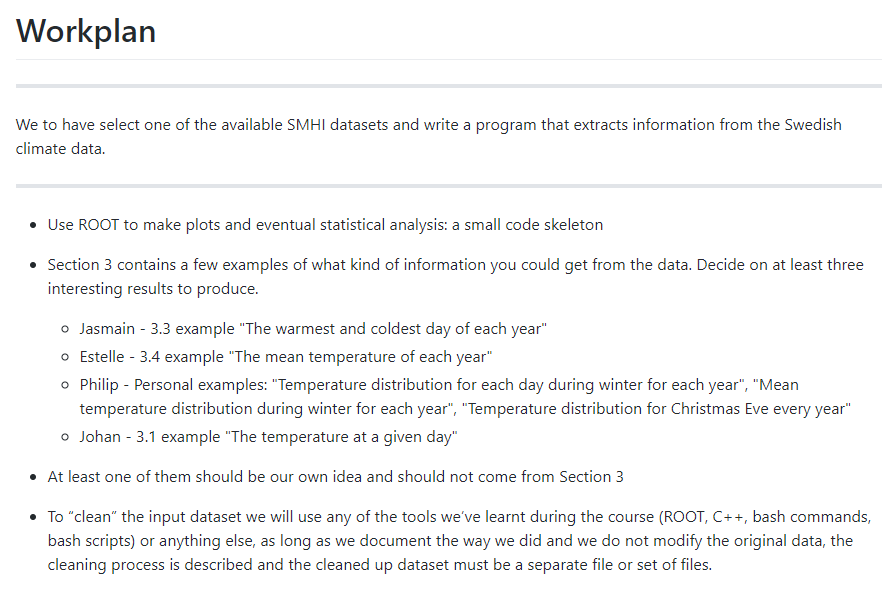
\includegraphics[scale=0.8]{Workplan.PNG}~\\[2cm]
\end{center}


\newpage
Then, we had to work on the datasheet we where interested in to make the access to it's content easier. It have of course been done via a program and there is a comparison before/after the program went through it :

~\\
\begin{center}
\textbf{Before} 
~\\
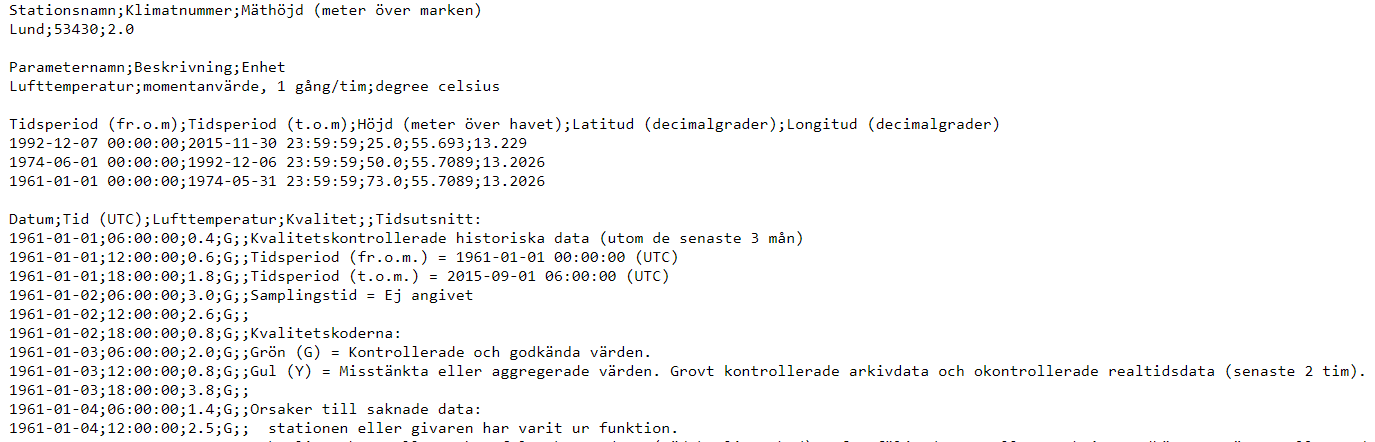
\includegraphics[scale=0.8]{DataSheetBefore.PNG}~\\[2cm]
\end{center}
\begin{center}
\textbf{After} 
~\\
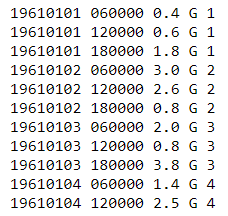
\includegraphics[scale=0.8]{DataSheetAfter.PNG}~\\[2cm]
\end{center}
So what been done is that all the useless information (in our case) have been removed as well as the ponctuation between the important inforamations (date, time , temperature etc). As a result we get a refined datasheet, with only blank space between the information, what makes it very easy to manipulate.

\newpage


















\end{document}